\lstset{ %
language=[Auto]Lisp,
basicstyle=\footnotesize,
frame=single,
numbers=left,
breaklines=true,
framerule=0.4mm,
showstringspaces=false}

\begin{appendices}
  \chapter{Primeira Versão}
  \label{chap:versao1}
  \lstinputlisting{/home/kaiser/Dropbox/monografia/code/versao1_monograph.clj}

  \chapter{Segunda Versão}
  \label{chap:versao2}
  \lstinputlisting{/home/kaiser/Dropbox/monografia/code/versao2_monograph.clj}

  \chapter{Terceira Versão}
  \label{chap:versao3}
  \lstinputlisting{/home/kaiser/Dropbox/monografia/code/versao3_monograph.clj}

  \chapter{Aproximações}
  \label{chap:aproximacao}
%  \begin{landscape}
  \begin{figure}[htb!]
    \begin{center}
      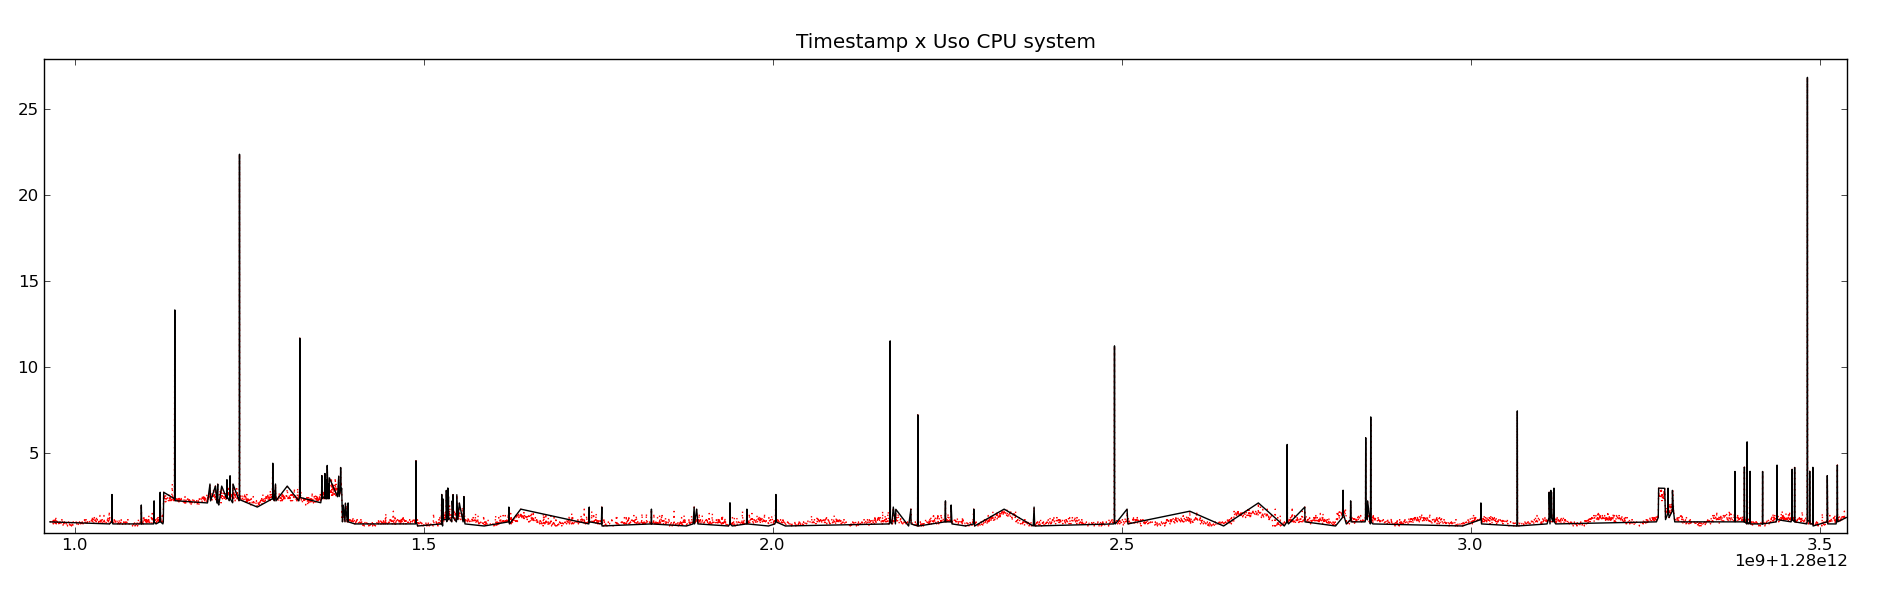
\includegraphics[width=1\textwidth]{timestampxcpu_system_8582_300_hpg-spo-squid-01}
      \centering
      \caption[Série original com 8582 pontos reduzida com PIP para 300 pontos]{Série original -- linha pontilhada em vermelho -- com 8582 pontos representando 1 mês de observações, reduzida com PIP para 300 pontos. Descarte de 99.976\% dos pontos originais.}
    \label{fig:approx1}
    \end{center}
  \end{figure}
%  \end{landscape}

\end{appendices}
